\subsection{KNN}
El análisis sobre el algoritmo $KNN$ ($k$ vecinos más cercanos) se realiza para distintos valores de $k$, fijando un valor de $\lambda$. La idea detrás de esta elección de variables busca entender la variación en la efectividad (cantidad de aciertos) del algoritmo.
Vamos a probar el algoritmo KNN para los siguientes valores:

$\alpha$: 10  y $k$: 1, 5, 20, 50, 250.\\

Además decidimos ejecutar por cada uno de los valores anteriores 5 pruebas iguales, esta decisión se debe a que el algoritmo varía la cantidad de aciertos dependiendo de la base de datos que analice y no siempre da el mismo resultado.

El procedimiento de este algoritmo comienza, por cada imágen que queremos averiguar a que dígito pertenece, con su vectorización. Luego resta el resultado a cada uno de los vectores imágen y calcula la norma 2 para saber en cuanto difieren con cada una de las imágenes.
Todos esos resultados se acumulan en una cola de prioridad que los ordena de menor a mayor, según las diferencias entre la imágen la cual se quiere averiguar a que clase pertenece y todas las imágenes de la base de datos etiquetada.
\\
Como siguiente paso se toman los $k$ primeros elementos de la cola de prioridad y se verifica a que dígito se corresponden para luego saber cual es el dígito que recibió mas \"votos\" y ver si se produjo un acierto o no.
Por lo tanto, a mayor cantidad de vecinos (o sea, $k$) menor va a ser la cantidad de aciertos, ya que se empiezan a mirar los elementos de menor prioridad de la cola, eso significa, que se cuentan primero las imágenes que más difieren y eso puede hacer que las chances de acertar el dígito correcto disminuyan.
\\
El algoritmo $KNN$ es muy efectivo ya que tiene aproximadamente entre 85\% y 90\% de aciertos. Pero su \"déficit\" es que es muy lento a comparación del algoritmo $PCA$. 

\subsubsection{Cantidad de vecinos}
Para analizar cual es el mejor número de vecinos para el cual el algoritmo $KNN$  da una mayor cantidad de aciertos, optamos por variar justamente la cantidad de $k$ vecinos a tomar.

Se prueba entonces el algoritmo $KNN$ para los siguientes valores:\\
$k$: 1, 5, 20, 50, 250.\\

A continuación vamos a mostrar los resultados para los valores reci\'en mencionados en forma de gráficos.

Una de las particularidades que podemos observar es que a menor cantidad de vecinos recorridos, mayor es la cantidad de aciertos, ya que como se eligen los mejores de la cola de prioridad, se obtiene mayor precisión debido a que los primeros elementos de la cola son los que menos difieren de las imágenes de la base de datos.
Por lo tanto, eligiendo $k = 1$ se obtiene la imagen del dígito que más cerca estuvo de la imagen pasada por parámetro, con lo cual no resulta relevante conocer cuales son los resultados de las siguientes imágenes de la cola ya que el primero es el mejor caso posible.

\subsection{PCA}
\subsubsection{Cantidad de vecinos y $\alpha$ inicial}
Vamos a probar el algoritmo para distintas medidas de $k$ y $\alpha$, que van a ser:\\
$k$: cantidad de vecinos a considerar en el algoritmo $kNN$.\\
$\alpha$: a la cantidad de componentes principales a tomar.

Vamos a probar el algoritmo para los siguientes valores:\\ \\
$\alpha$: 10  y k: 5, 20.\\
$\alpha$: 200 y k: 5, 20.\\
$\alpha$: 700 y k: 5, 20.\\
$\alpha$: 50  y k: 5, 25, 50, 100.\\

La prueba a realizar es, fijando un valor de $\alpha$, analizar para que cantidad de vecinos se obtiene la mayor cantidad de aciertos y así maximizar la cantidad de aciertos totales.
Después de aplicar el algoritmo $PCA$, se aplica el algoritmo $KNN$, armando una cola de prioridad para los resultados de aplicar el algoritmo $KNN$. Lo que se hace es tomar dos imágenes, restarlas y aplicarle la norma 2 para saber en cuanto difiere una imagen de la otra. En la cola de prioridad se encuentran por delante los valores más chicos, o sea, las imágenes del test que más cerca de coincidir están con respecto a la imágen de la base de datos.
Por lo tanto, si elegimos una mayor cantidad de vecinos, pueden pasar dos cosas:

\begin{itemize}
  \item Que sea beneficioso ya que a mayor cantidad de pruebas vamos a tener mas aciertos
  \item Que sea malicioso ya que a mayor cantidad de pruebas vamos a obtener peores datos, o sea, vamos a mirar las imágenes que menos coiciden con la imagen de prueba de la base de datos.
\end{itemize}

Además, enfocamos nuestro análisis en obtener un valor óptimo de $\alpha$. Para este fin, realizamos varias corridas tratando de maximizar la performance del algoritmo. Dado que este parámetro representa la cantidad de componentes principales a tener en cuenta y teniendo en mente el funcionamiento del algoritmo de PCA, es esperable que valores pequeños no sean beneficiosos (teniendo en cuenta que el máximo a considerar es bastante elevado), pero dado que PCA las ordena en base a su relevancia, se alcance un valor óptimo sin necesidad de considerarlas todas. A continuación presentamos algunas de las mediciones realizadas.

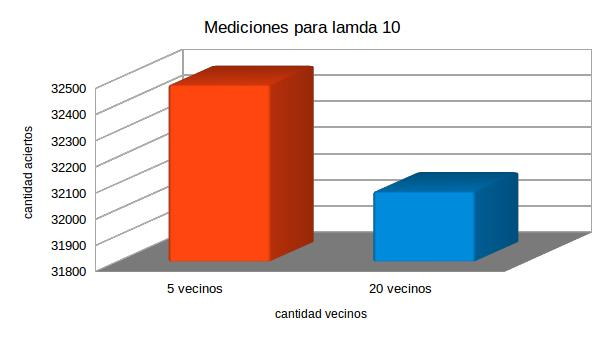
\includegraphics[scale=0.75]{lamda10.jpg}\\
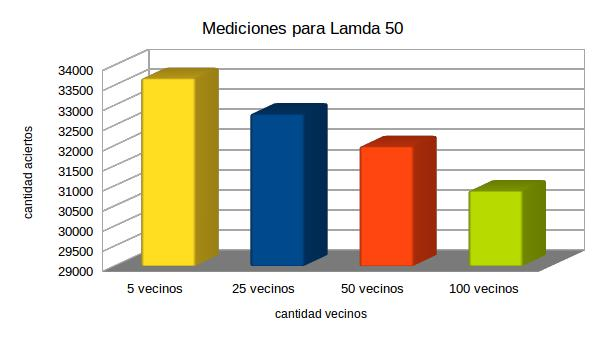
\includegraphics[scale=0.75]{lamda50.jpg}\\
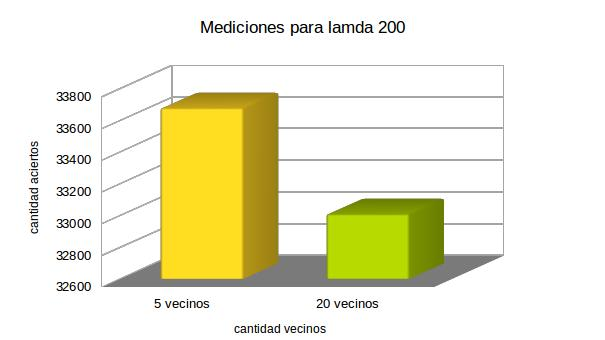
\includegraphics[scale=0.75]{lamda200.jpg}\\
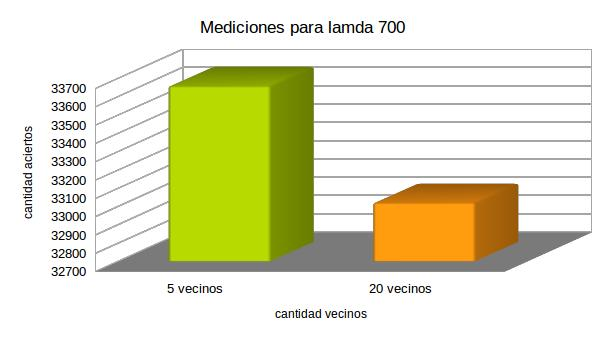
\includegraphics[scale=0.75]{lamda700.jpg}\\

En la primera corrida, con un valor mínimo de $\alpha$ (seteado en 10) se obtiene un resultado cercano a los 32,200 aciertos. A medida que este valor se aumenta, se puede apreciar como se obtiene una mejora considerable, cercana a los 33,000 aciertos, pero como enseguida se alcanza un máximo y sin importar cuantas más componentes se tengan en cuenta para la ejecución, no se presenta una mejora significativa de los resultados. En cuanto a la cantidad de vecinos, como quedo demostrado con anterioridad, se sigue repitiendo el mismo patrón esperado: a mayor cantidad considerada, el algoritmo empieza a funcionar peor, ya que estamos mirando los vecinos que menos coinciden con la base de datos, debido a que la cola de prioridad los ordena según la menor cantidad de diferencias entre la imagen obtenida y las imágenes de la base de datos. 
Es importante destacar que se realizaron 10 corridas para cada variación del parámetro utilizando el algoritmo de cross-validation para minimizar los sesgos producidos por el sobre ajustamiento de los parámetros y se promediaron los resultados.

%Otra conclusión que sacamos es que $k = 5$ vecinos es la mejor cantidad de vecinos para obtener la mayor cantidad %de aciertos. 
%Ahora, ¿No sería mejor agarrar solo el primero de la cola de prioridad, es decir, $k = 1$? 
%Lo que podría pasar es que el único vecino que utilicemos sea el mejor pero no alcance para saber cuál es el %dígito de la imagen, ya que si no se acierta con el único vecino que se elije,  podría fallar el dígito del %resultado, reduciendo en un alto grado la cantidad de aciertos.
